\documentclass[a4paper,10pt]{report}
\usepackage[utf8]{inputenc}
\usepackage{fancyhdr}
\usepackage[french]{babel}
\usepackage[authoryear, numbers]{natbib}
\usepackage[final]{pdfpages} 
\lhead[\rm\thepage]{\fancyplain{}{\sl{\rightmark}}}
\rhead[\fancyplain{}{\sl{\leftmark}}]{\rm\thepage}





\begin{document}
\title  {Titre du papier}
\author  {Thibault François }
\maketitle
%\lhead{\emph{Table des matières}}  % Set the left side page header to "Contents"
\tableofcontents  % Write out the Table of Contents

\chapter{Introduction}
\chapter{Définition du contexte}
\section{Structure le l'organisation}
\section{Existant : les problèmes lié à l'existant, comment on veut les résoudre}

\chapter{Elaboration du référentiel de compétence}
\chapter{Comment évaluer les compétences}
\chapter{Mise en oeuvre}
\chapter{Conclusion}
\section{Critique de la gestion des compétences et }

\chapter*{Introduction}

 % Sigle et Abréviation + Résumé + Introduction


\chapter{Contexte} \label{contexte}






%\lhead{\emph{Conclusion}}


\label{Bibliographie}
\lhead{\nouppercase{\leftmark}}
\bibliographystyle{unsrtnat}  % Use the "unsrtnat" BibTeX style for formatting the Bibliography
\bibliography{Bibliography} 



%% ----------------------------------------------------------------
% Now begin the Appendices, including them as separate files
\part*{Annexes}
\lhead{\nouppercase{\leftmark}}
\appendix % Cue to tell LaTeX that the following 'chapters' are Appendices

%\input{./Appendices/AppendixA}	% Exigences

\chapter{Odoo Appraisal Form}
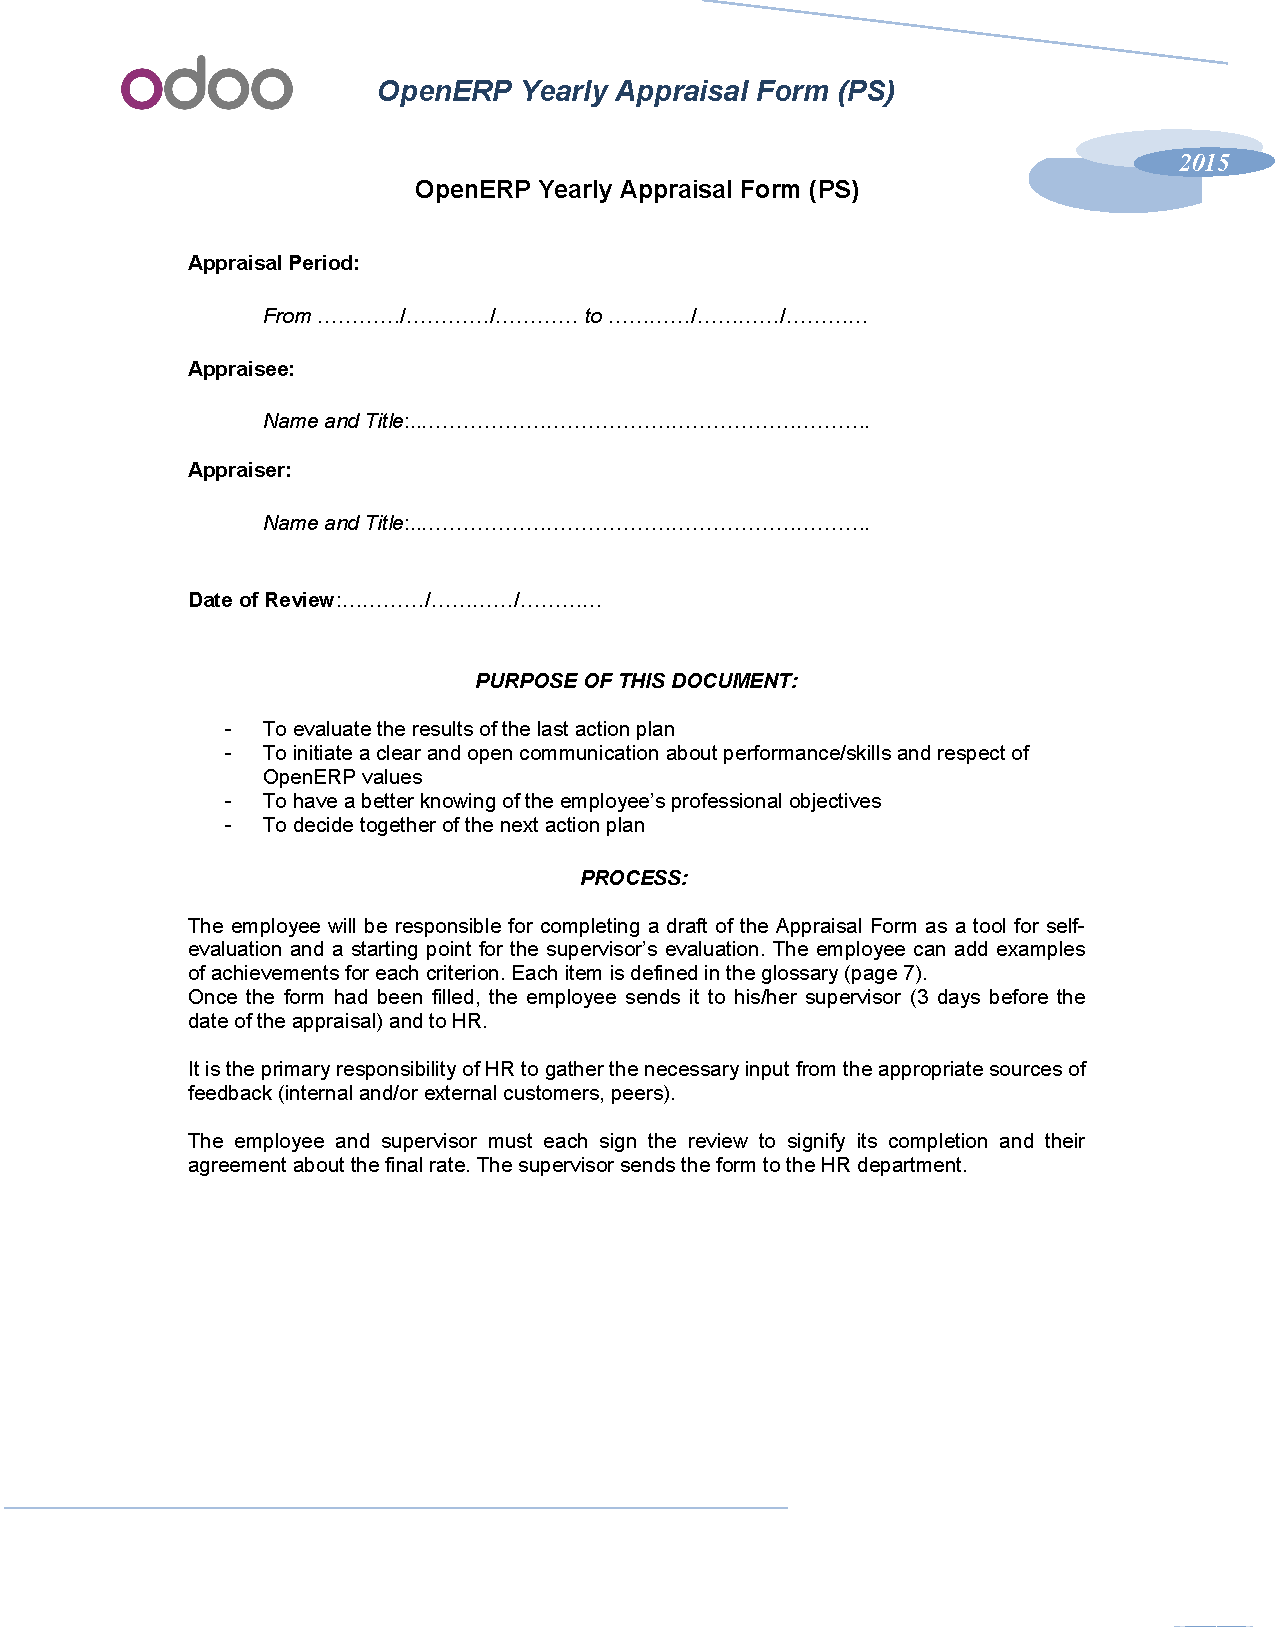
\includepdf[pages=1-6]{document/Odoo_appraisal.pdf}

\addtocontents{toc}{\vspace{2em}}  % Add a gap in the Contents, for aesthetics



\end{document}
